%%% LaTeX Template: Designer's CV
%%%
%%% Source: http://www.howtotex.com/
%%% Feel free to distribute this template, but please keep the referal to HowToTeX.com.
%%% Date: March 2012


%%%%%%%%%%%%%%%%%%%%%%%%%%%%%%%%%%%%%
% Document properties and packages
%%%%%%%%%%%%%%%%%%%%%%%%%%%%%%%%%%%%%
\documentclass[a4paper,12pt,final]{memoir}

% misc
\renewcommand{\familydefault}{bch}	% font
\pagestyle{empty}					% no pagenumbering
\setlength{\parindent}{0pt}			% no paragraph indentation


% required packages (add your own)
\usepackage{flowfram}										% column layout
\usepackage[top=1cm,left=0.2cm,right=1cm,bottom=0.8cm]{geometry}% margins
\usepackage{graphicx}
\usepackage{epstopdf} 									% figures
\usepackage{url}											% URLs
\usepackage[usenames,dvipsnames]{xcolor}					% color
\usepackage{multicol}										% columns env.
	\setlength{\multicolsep}{1pt}
\usepackage{paralist}										% compact lists
\usepackage{tikz}
\usepackage{textcomp}

%\usepackage{anyfontsize}
\usepackage[hidelinks]{hyperref}

%%%%%%%%%%%%%%%%%%%%%%%%%%%%%%%%%%%%%
% Create column layout
%%%%%%%%%%%%%%%%%%%%%%%%%%%%%%%%%%%%%
% define length commands
\setlength{\vcolumnsep}{\baselineskip}
\setlength{\columnsep}{\vcolumnsep}

% frame setup (flowfram package)
% left frame
\newflowframe{0.265\textwidth}{\textheight}{0pt}{0pt}[left]
	\newlength{\LeftMainSep}
	\setlength{\LeftMainSep}{0.2\textwidth}
	\addtolength{\LeftMainSep}{4\columnsep}

% right frame
\newflowframe{0.7\textwidth}{\textheight}{\LeftMainSep}{0pt}[main01]

% horizontal rule between frames (using TikZ)
\renewcommand{\ffvrule}[3]{%
\hfill
\tikz{\draw[loosely dotted,color=Plum,line width=1.5pt,yshift=-#1](0, 0) -- (0pt,#3);}
\hfill\mbox{}}
\insertvrule{flow}{1}{flow}{2}


%%%%%%%%%%%%%%%%%%%%%%%%%%%%%%%%%%%%%
% define macros (for convience)
%%%%%%%%%%%%%%%%%%%%%%%%%%%%%%%%%%%%%
\newcommand{\Sep}{\vspace{1.5em}}
\newcommand{\SmallSep}{\vspace{0.5em}}

\newenvironment{Objective}
	{\ignorespaces\textbf{\color{Plum} Objective}}
	{\Sep\ignorespacesafterend}
	
\newcommand{\CVSection}[1]
	{\Large\textbf{#1}\par
	\SmallSep\normalsize\normalfont}

\newcommand{\CVItem}[1]
	{\textbf{\color{Plum} #1}}

%\urlstyle{}

%%%%%%%%%%%%%%%%%%%%%%%%%%%%%%%%%%%%%
% Begin document
%%%%%%%%%%%%%%%%%%%%%%%%%%%%%%%%%%%%%
\begin{document}

% Left frame
%%%%%%%%%%%%%%%%%%%%
%\begin{figure} 
%	\hfill
%	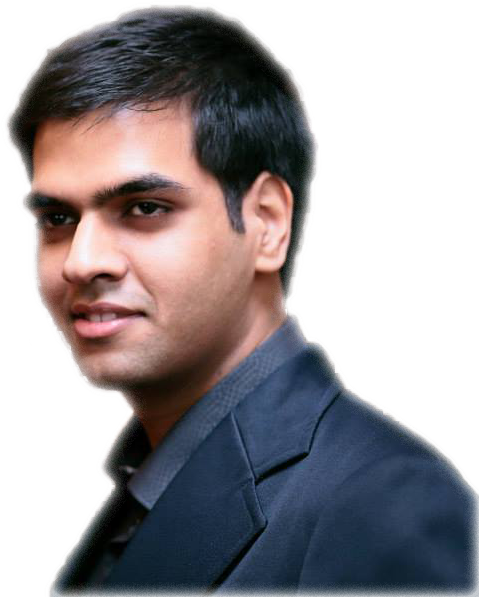
\includegraphics[width=0.8\columnwidth]{kkk}
%	\vspace{-5cm}
%\end{figure}

\begin{flushright} 
	\footnotesize
	\SmallSep
	{\bfseries{\color{Plum}{Address}}}\\
	
	105 NW 103rd St\\
	Seattle, WA - 98177\\
	\Sep
	{\bfseries{\color{Plum}{EMail}}}\\
	\href{mailto:vicky.p.katara@gmail.com}{vicky.p.katara@gmail.com}\\
	\Sep
	{\bfseries{\color{Plum}{Cellphone}}}\\
	\href{tel:+19842158067}{+1 \(984\)215-8067}\\
	\Sep
		%{\bfseries{\color{Plum}{Website}}}\\
	%\href{http://vickykatara.orgfree.com/}{vickykatara.orgfree.com}\\
\end{flushright}\normalsize
%\begin{figure}
	%\hfill
	%\vspace{-0.3cm}
	\hspace{0.9cm}
		\vspace{-0.35cm}
	\bfseries{\color{Plum}{Save My Contact}}\\\\
	\vspace{-0.1cm}
	\hspace{-0.4cm}
	
\includegraphics[width=0.8\columnwidth]{qrcode_2.eps}
%\end{figure}
\framebreak

% Right frame
%%%%%%%%%%%%%%%%%%%%

\normalsize\normalfont

\CVSection{Projects(continued)}
%Project-3 Start
\CVItem{Design, Development and Deployment of Personal Website}\\
{\footnotesize Configuration, maintenance of personal website. Also involved content writing.\\\emph{Technologies Used:} HTML / JavaScript / CSS / Wordpress}%Project-3 End
\SmallSep\\
%Project-1 Start
\CVItem{Development of Mini-Tennis Game, Mini-Project for Computer Graphics}\\
{\footnotesize This involved the design and development of 2D Mini-Tennis game.\\ \emph{Technologies Used:} GCC / graphics.l}\\%Project-5 End
%\Sep
 
% Projects - End
% Skills
\CVSection{Skills}
\CVItem{Programming Languages}\\
{\footnotesize Java, C/C++, PL/SQL, Python, Ruby}
\SmallSep\\
\CVItem{Web Technologies}\\
{\footnotesize HTML, CSS, JavaScript, Ruby on Rails}
\SmallSep\\
\CVItem{Database Platforms}\\
{\footnotesize Oracle 9i / 11g, MySQL, SQL Server, MS Access}
\SmallSep\\
\CVItem{Applications}\\
{\footnotesize Informatica PowerCenter, SQL Developer, Toad, Adobe Photoshop, NetBeans, VMWare, Oracle Hyperion, IBM Cognos Report Studio, Audacity, MS Office, \LaTeX}
\SmallSep\\
\CVItem{Operating Systems}\\
{\footnotesize Microsoft Windows(98/XP/7/8), Linux, Android}
\SmallSep\\
\CVItem{Certifications}\\
{\footnotesize Oracle Certified Java SE6 Programmer(scored 93 \%)}
\Sep

% Awards and Achievements
\CVSection{Awards and Achievements}
\CVItem{Awards}\SmallSep\\
\begin{minipage}{13.5cm}
	\begin{compactitem}[\color{Plum}$\circ$]
		{\footnotesize
			\item Received SPOT Award while working with Deloitte
			\item Received Student of the Year in the senior year of High School}
	\end{compactitem}
\end{minipage}
\SmallSep\\
\CVItem{Achivements}\SmallSep\\
\begin{minipage}{13.5cm}
	\begin{compactitem}[\color{Plum}$\circ$]
		{\footnotesize
			\item Conducted workshop on Java in April 2012, with ISTE-TSEC
			\item Won consolation prize In Java Based Programming Competition
			\item Level 2 member On ProjectEuler.net, ranked 172 in India}
	\end{compactitem}
\end{minipage}
\Sep\\

% Additional
\CVSection{Additional Information}
\CVItem{Community Service}\SmallSep\\
\begin{minipage}{13.5cm}
	\begin{compactitem}[\color{Plum}$\circ$]
		{\footnotesize
			\item Personal tutoring to students from impoverished backgrounds
			\item Regularly participate in Animal welfare campaigns in and around Mumbai
			\item Helped spread awareness and participated in cleanliness campaigns in impoverished tribal localities}
	\end{compactitem}
\end{minipage}
\SmallSep\\
\CVItem{Extracurricular Activities}\SmallSep\\
\begin{minipage}{13.5cm}
	\begin{compactitem}[\color{Plum}$\circ$]
		{\footnotesize
			\item Elected Event Head for treasure hunt event organised By TSF
			\item Selected science project group leader at the inter-school level
			\item Appointed House Captain for two academic years in High School}
	\end{compactitem}
\end{minipage}
\SmallSep\\
\CVItem{Hobbies and Interests}\SmallSep\\
\begin{minipage}{13.5cm}
	\begin{compactitem}[\color{Plum}$\circ$]
		{\footnotesize
			\item Playing Football(Soccer)
			\item Solving problems on Plane Geometry
			\item Mathematical / Algorithmic Programming and Puzzle Solving}
	\end{compactitem}
\end{minipage}
\Sep\\

%%%%%%%%%%%%%%%%%%%%%%%%%%%%%%%%%%%%%
% End document
%%%%%%%%%%%%%%%%%%%%%%%%%%%%%%%%%%%%%

\end{document}